\documentclass[a4paper,10pt, spanish]{article}

\usepackage{graphicx}
\usepackage{listings}
\usepackage[final]{pdfpages}
\usepackage[spanish]{babel}
\usepackage[utf8]{inputenc}
\usepackage[export]{adjustbox}
\usepackage{mips}

\lstset{
language=C,
tabsize=2,
  basicstyle=\small\ttfamily,
  columns=fullflexible,
  frame=single,
  breaklines=true,
  resetmargins=true
}

\title{
            \large{Organización de Computadoras} \\
            \textbf{Trabajo Práctico 1} \\
            \textbf{Implementación en MIPS Assembly} \\
            \bigskip
            
\includegraphics[max height=100pt,max width=100pt]{./UBA.png} \\
}

\author{	Nicolás Ledesma, \textit{Padrón Nro. 93.118}                        \\
            \texttt{ nicolas.angel.ledesma@gmail.com }                           \\[2.5ex]
            Jonathan Moguilevsky, \textit{Padrón Nro. 95.516}                   \\
            \texttt{ jmoguilevsky@gmail.com }                                   \\[2.5ex]
            Leonardo Riego, \textit{Padrón Nro. 94.104}                 \\
            \texttt{ riegoleonardo@hotmail.com }                                          \\[2.5ex]
            \normalsize{2do. Cuatrimestre de 2019}                              \\
            \normalsize{66.20 Org. de Computadoras
                $-$ Práctica: Santi, Pérez Masci, Natale }                      \\
            \normalsize{Facultad de Ingeniería, Universidad de Buenos Aires}    \\
       }
\date{}

\begin{document}

\maketitle

\thispagestyle{empty}   % quita el número en la primer página


\begin{abstract}
Este trabajo práctico grupal tiene como objetivo poner en práctica los conocimientos adquiridos sobre la arquitectura MIPS y la programación en assmebly en este entorno. Asimismo, se ponen en práctica la convenciones de código dispuestas por la MIPS ABI.
\end{abstract}

\pagebreak

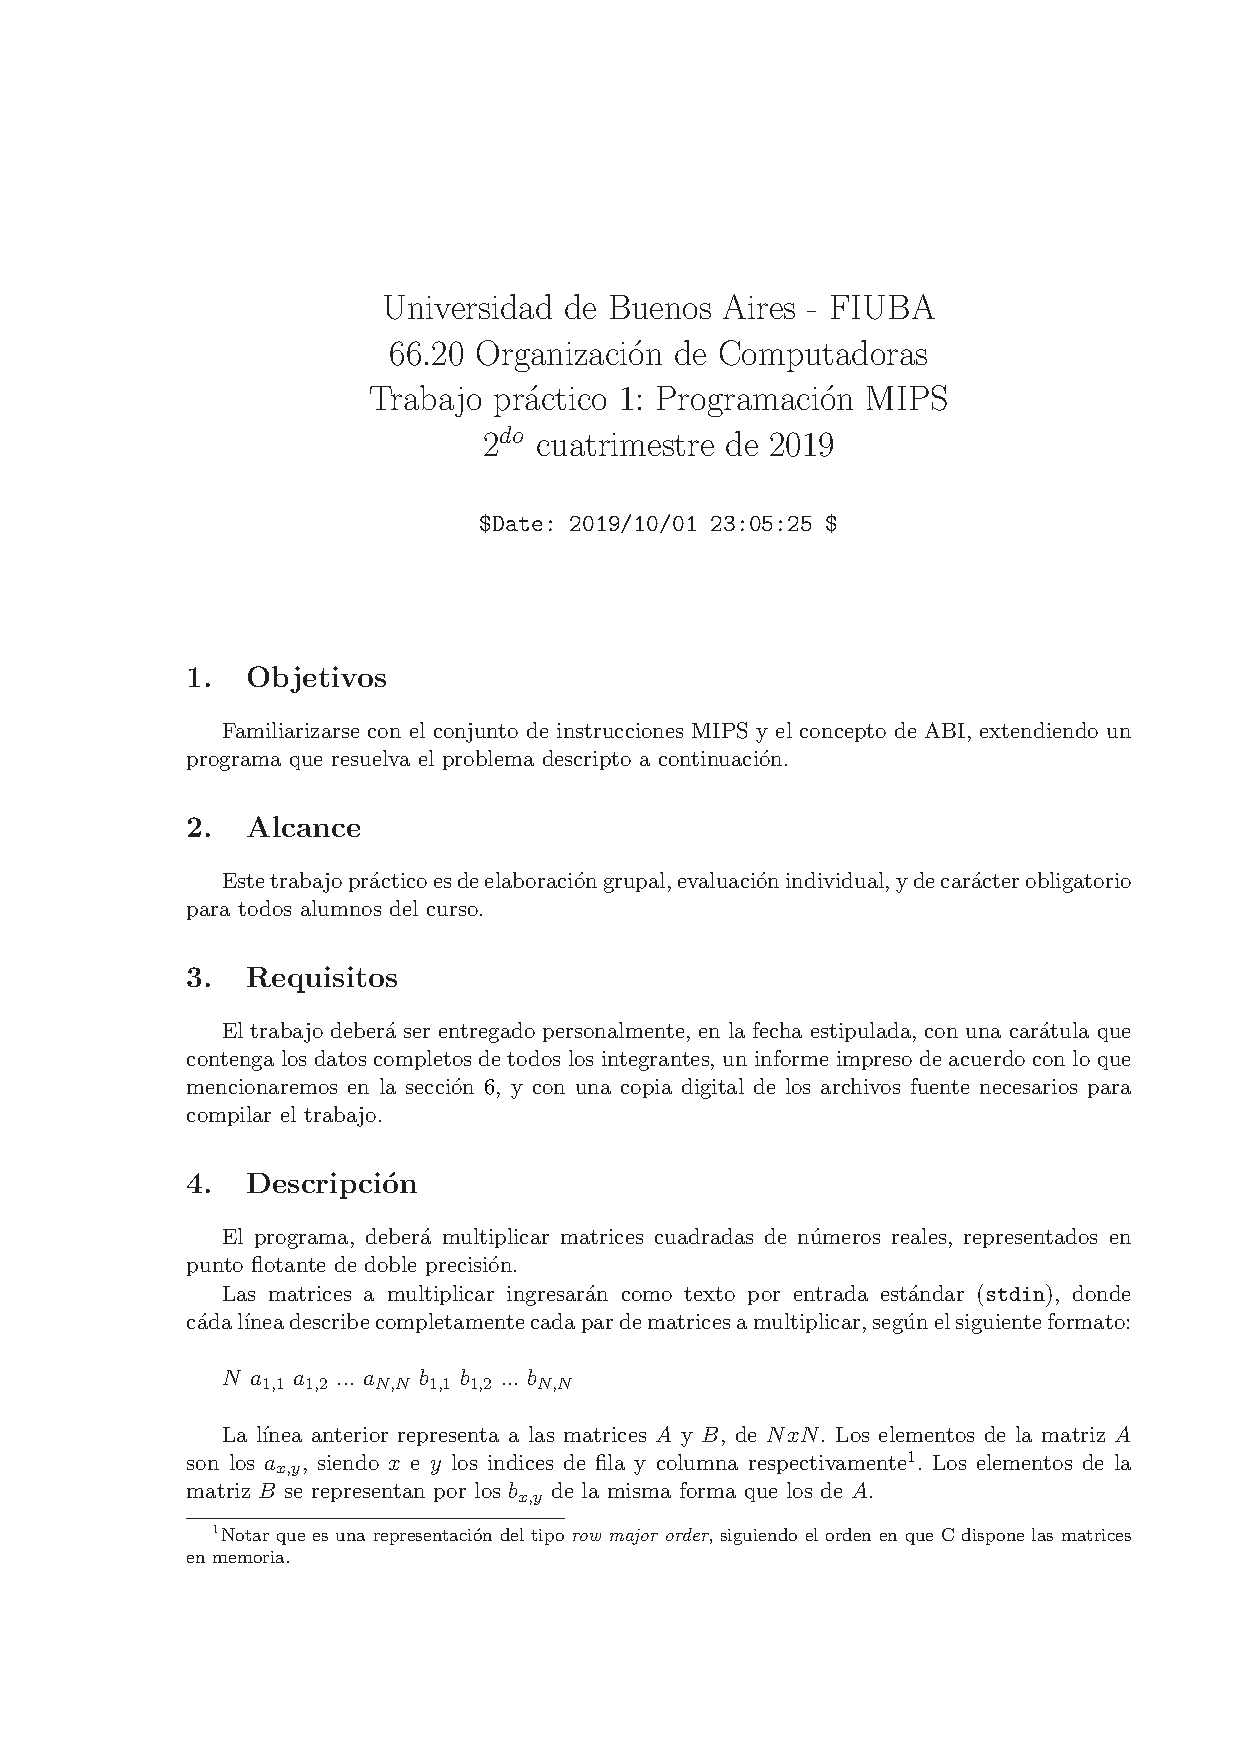
\includepdf[
    trim=20mm 30mm 10mm 25mm, clip,
    pages=1,
    frame,
    scale=.65,
    pagecommand=\section{Enunciado}
 ]{./tp1-2019-2q.pdf}
\includepdf[
    trim=20mm 30mm 10mm 25mm, clip,
    pages=2-,
    frame,
    scale=.65,
    pagecommand={}
 ]{./tp1-2019-2q.pdf}

\section{Solución}

\subsection{Diseño}
Algunos fragmentos del código entregado en el trabajo práctico anterior se mantienen sin modificaciones:
\begin{itemize}
  \item Se conserva el código escrito para las funciones de lectura y procesamiento del input para generar las matrices de entrada, y para imprimir los resultados de la multiplicación.
  \item También se mantiene sin cambios la presentación de menus y mensajes de error.
\end{itemize}

A fines de reservar y liberar memoria alocada para matrices en forma compatible con el código assembly, las funciones \textbf{create\_matrix} y \textbf{destroy\_matrix} de C ahora utilizan las rutinas \textbf{my\_malloc} y \textbf{my\_free} definidas en el archivo \textbf{my\_malloc.S}. 

Por otra parte, se implementaron en lenguaje assembly de MIPS las funciones \textbf{matrix\_multiply} y \textbf{create\_matrix\_S}

Si bien se mantiene una versión del código C de \textbf{create\_matrix}, la nueva versión en assembly es empleada internamente dentro de la función \textbf{matrix\_multiply} para generar la matriz resultado.

\subsubsection{matrix\_multiply}

Esta función se encarga del cálculo del producto de las matrices ingresadas. Fue implementada siguiendo el mismo procedimiento que la versión previa escrita en lenguaje C. 

La principal diferencia con el código C anterior es que internamente esta función llama a la implementación de \textbf{create\_matrix\_S} escrita en assembly.\\

\lstinline{Stack frame} \\
            \begin{center}
              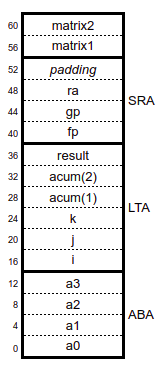
\includegraphics[max height=100pt,max width=100pt]{./stack_matrix_multiply.png}
            \end{center}
            \begin{itemize}
                \item \lstinline{SRA}
                Se guardaron los registros gp, fp y ra en este área, con 4 bytes de padding para que quede alineada a 8 bytes como dicta la ABI
                \item \lstinline{LTA}
                Se reservaron espacios de memoria para las variables i, j y k que son los contadores utilizados en los distintos loops, 8 bytes para la variable acum utilizada para guardar los resultados parciales, y result que es utilizado como puntero a la estructura que guarda el resultado final.
            \end{itemize}

           Además, se definieron las constantes STACK\_SIZE(tamaño del stack), OFFSET\_RA, OFFSET\_FP y OFFSET\_GP para los offsets de las posiciones de memoria donde se guardaran los registros ra, fp y gp respectivamente

\subsubsection{create\_matrix\_S}
    Función encargada de reservar memoria para una matriz con las dimensiones recibidas por parametro.
    
    Esta función se encarga de alocar la memoria para la estructura que almacena la matriz resultado. Por ello internamente utiliza una rutina que reserva memoria en heap, llamada \textbf{my\_malloc}, en el archivo \textbf{my\_malloc.S}. 
    
    Cabe remarcar que la memoria alocada dentro de este código es luego liberada en el código C.\\
    \lstinline{Stack frame} \\
            \begin{center}
              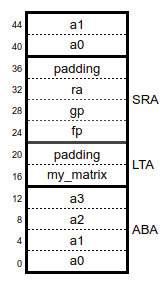
\includegraphics[max height=100pt,max width=100pt]{./stack_create_matrix.png}
            \end{center}
            \begin{itemize}
                \item \lstinline{SRA}
                Se guardaron los registros gp, fp y ra en este área, con 4 bytes de padding para que quede alineada a 8 bytes como dicta la ABI
                \item \lstinline{LTA}
                Se reserva una posicion en el stack donde se guardará la dirección de memoria de la matriz creada
            \end{itemize}
     Además, se definieron las siguientes constantes:
        \begin{itemize}
            \item \lstinline{STACK_SIZE_CREATE_MATRIX:} tamaño stack
            \item \lstinline{OFFSET_RA_CREATE_MATRIX:} offset ra
            \item \lstinline{OFFSET_GP_CREATE_MATRIX:} offset gp
            \item \lstinline{OFFSET_FP_CREATE_MATRIX:} offset fp
            \item \lstinline{OFFSET_MY_MATRIX_CREATE_MATRIX:} offset variable my\_matrix
            \item \lstinline{A0_CALLEE_CREATE_MATRIX:} offset primer registro ABA
            \item \lstinline{A0_CALLER_CREATE_MATRIX:} offset primer argumento de la función
            \item \lstinline{A1_CALLER_CREATE_MATRIX:} offset segundo agurmento de la funcion
        \end{itemize}


\subsection{Código}

\lstinputlisting{../dynamic.c}
\lstinputlisting{../matrix_multiply.S}

\lstset{
  language=bash,
  basicstyle=\small\ttfamily
}

\subsection{Compilación del programa}
Para compilar el programa se utiliza el makefile desde el directorio donde se descomprimió el entregable:
\begin{lstlisting}
$ make clean
$ make all
\end{lstlisting}

\section{Pruebas}

\subsubsection{Ejecución}

Para la ejecución de las pruebas generamos un script llamado \lstinline{run_tests.sh} que se encarga de, para cada caso generado, ejecutar el programa y escribit el output en un archivo.
Finalmente, se comparan los outputs contra archivos que contienen los resultados esperados, en la carpeta \lstinline{results/}.

\subsection{Casos de prueba}

Para probar nuestro programa generamos una serie de casos de prueba:

\begin{itemize}
  \item \lstinline{big_matrix_ints.txt:} Matriz de 100x100 con valores enteros
	\item \lstinline{big_matrix_doubles.txt:} Matriz de 100x100 con valores de punto flotante
  \item \lstinline{exponential_doubles_matrix.txt:} Matriz pequeña con valores de punto flotante en notación exponencial.
  \item \lstinline{invalid_input.txt:} Prueba con input invalido.
  \item \lstinline{simple_multiline.txt:} Prueba de input con varias líneas.
  \item \lstinline{single_line.txt:} Prueba simple de una sola línea.
  \item \lstinline{small_double_matrix.txt:} Prueba simple de una matriz 3x3 de doubles.
  \item \lstinline{small_int_matrix.txt:} Prueba simple de una matriz 3x3 de integers.
\end{itemize}

La ejecución de los casos se realiza de la siguiente manera:

\begin{lstlisting}
$ ./run_tests.sh
\end{lstlisting}

Este script de ejecución valida también la impresión del menú y de la versión del programa.

\section{Conclusiones}

En este trabajo pusimos en práctica la definición de un programa en MIPS assembly, lo cual nos lleva a los siguientes aprendizajes y conclusiones:

\begin{itemize}
  \item Al definir y crear el stack frame dentro de cada función que implementamos, se tiene pleno control (sin olvidar respetar la ABI) y conocimiento del uso de la memoria principal del programa.
  \item Se observa a su vez que las gestión de recursos de la máquina es absoluta, tanto en el uso de memoria como de los registros del procesador.
  \item Resulta tedioso al principio valerse de menos herramientas al encontrarnos desarrollando en tan bajo nivel y en un entorno de desarrollo tan cerrado como la máquina virtual con el sistema operativo NetBSD.
  \item La herramienta de debugging gdb resultó ser muy util a la hora de diagnosticar comportamientos indeseados en el programa en la medida que lo construimos. Permite visualizar de una forma muy práctica los registros y direcciones utilizados en tiempo real durante la ejecución del programa.
\end{itemize}

\end{document}
